
\section{Introduction}
Comme nous l'avons présenté dans le premier chapitre à travers la section \ref{Archi1} et la section \ref{Archi2}, il existe deux approches pour développer un système de reconnaissance de la parole : l'approche basée reconnaissance de phonèmes et l'approche End-To-End; chacune présente un intérêt pour notre problématique, qui est la conception et le développement d'un système de reconnaissance de la parole pour la langue arabe. Le choix de l'approche se fait à travers l'étude des avantages et inconvénients, dans le contexte général puis dans le contexte de ce projet particulièrement, suivie d'une phase d'expérimentations pour appuyer notre raisonnement.

Nous présentons en premier lieu dans ce chapitre un comparatif de ces deux approches et nous justifions notre choix. Nous poursuivons par l'étape de collecte des données que nous utiliserons pour l'apprentissage de \textit{ASeR-System (\textbf{A}rabic \textbf{S}pe\textbf{e}ch \textbf{R}ecognition System)}, notre système de reconnaissance de la parole. Nous détaillons par la suite les différentes architectures que nous avons utilisées pour nos expérimentations ainsi que la méthodologie suivie pour définir les différentes architectures de ce système. 

\section{Choix de l'approche pour la conception de ASeR-System}
Afin de choisir l'approche que nous allons utiliser pour développer notre système de reconnaissance de la parole, nous étudions les avantages et inconvénients de l'approche End-To-End ainsi que l'approche basée reconnaissance de phonèmes en nous basant sur des critères que nous présentons ci-dessous. Nous commençons par comparer les corpus que nous utiliserons pour chacune des deux approches.

\subsection{Corpus utilisé}
Développer un système de reconnaissance de la parole End-To-End requiert une grande quantité de données par rapport à l'approche basée reconnaissance de phonèmes pour que le modèle puisse comprendre la structure morphologique de la langue. Cependant, la collecte de données pour l'approche End-To-End est plus intuitive car pour former un corpus. En effet, il suffit de récupérer des enregistrements audio et leurs transcriptions ce qui facilite grandement la collecte de données et l'enrichissement des corpus.

Le corpus utilisé pour l'approche basée reconnaissance de phonèmes quant à lui doit contenir les descriptions phonétiques des transcriptions. Il doit également contenir les informations temporelles qui sont les temps de début et de fin de chaque phonème ce qui peut s'avérer plus difficile à préparer.

\subsection{Comparaison des performances}
Nous avions noté dans la présentation de l'état de l'art que les systèmes basés reconnaissance de phonèmes les plus performants tel que Dragon Mobile SDK ou encore Google Speech API présentent des taux d'erreur moin élevés que les systèmes End-To-End. Ceci est dû à la qualité des corpus phonétiques utilisés pour ces systèmes qui ne sont, la plupart du temps, disponibles qu'au sein des laboratoires qui les développent. Nous avons également noté qu'entre 2014, où les systèmes End-To-End furent introduits, et aujourd'hui, les performances de ces derniers se sont largement améliorés se rapprochant ainsi de la performance des systèmes basés reconnaissance de phonèmes. Ceci laisse à penser qu'à l'avenir, avec des corpus plus riches en terme de quantité de données, les systèmes End-To-End seraient aussi performants que l'humain en terme de reconnaissance de la parole. Cette intuition se base sur les performances de l'état de l'art que nous avons rapportées dans les sections \ref{stateartphoneme} et \ref{statearte2e} de ce document.

\subsection{Complexité de développement}
Le développement d'un système basé reconnaissance de phonèmes requiert :
\begin{itemize}
    \item une équipe de linguistes pour la collecte d'un corpus qui contient la description phonétique de chaque enregistrement audio. Cette tâche peut s'avérer complexe et fastidieuse,
    \item le développement d'un modèle acoustique en utilisant les HMMs combinés à des GMMs ou encore à des réseaux de neurones profonds ainsi qu'une connaissance approfondie de la structure morphologique de langue traitée ce qui nécessite un expertise supplémentaire, et
    \item le développement d'un modèle de langage pour corriger et/ou valider l'interprétation du modèle acoustique. \\
\end{itemize}

Comparé à l'approche basée reconnaissance de phonèmes, le développement d'un système End-To-End se limite à la collecte d'un corpus d'enregistrements et de transcriptions qui peut se faire à l'aide d'algorithmes et sans intervention humaine et au développement d'un modèle Séquence à Séquence\footnote{Séquence à Séquence : Traduit de l'anglais "Sequence To Sequence", est un paradigme pour le développement de modèles capable de prédire des données séquentielles.} en utilisant des techniques d'apprentissage profond.

\subsection{Capacité d'amélioration des performances}
Le bon développement de tout système nécessite que ce dernier soit simple à maintenir et à enrichir. Ce n'est pas forcément le cas d'un système basé reconnaissance de phonèmes où la collecte de données pour le modèle acoustique est une tâche fastidieuse qui nécessite l'intervention de linguistes.

À contrario, un système End-To-End est plus facile à entretenir et surtout à améliorer. En premier lieu, la collecte de données présente moins de difficultés et ne nécessite pas d'intervention humaine. En second lieu, les avancées des différentes techniques d'apprentissage profond et la communauté de développeurs derrière ces techniques font des systèmes End-To-End une approche plus répandue et plus sûre aujourd'hui.

\subsection{Discussion}
Nous déduisons à travers ce comparatif, que chacune des deux approches présente des avantages que l'autre n'a pas. L'approche basée reconnaissance de phonèmes présente de meilleurs résultats avec un corpus moins volumineux grâce aux descriptions phonétiques mais la génération de tels corpus et leur enrichissement est une tâche difficile.
Les systèmes End-To-End quant à eux, ne nécessitent pas de descriptions phonétiques pour les corpus, ce qui facilite grandement leur enrichissement et donc l'amélioration des performances de ces systèmes. En plus des données, le développement d'un système End-To-End repose sur des techniques plus performantes et mieux documentées.

Notre choix s'est donc porté sur le développement d'un système de reconnaissance de la parole End-To-End. Dans la suite de ce chapitre, nous présentons les techniques que nous avons utilisées dans ce projet ainsi que les différentes architectures possibles pour ce développement. Nous commençons la conception de notre système par la collecte des données nécessaires à l'apprentissage de nos modèles.

\section{Environnement de développement pour la reconnaissance de la parole}
Dans le cadre de ce projet, nous développons notre propre système End-To-End de reconnaissance de la parole. En plus de ce système, nous nous attelons à la création d'un environnement de développement permettant à toute personne de non seulement utiliser notre système, mais aussi et surtout de contribuer à son amélioration. Cette initiative est motivée par le fait que la recherche dans le domaine de la reconnaissance de la parole et la compréhension du langage naturel est des plus actives. Ainsi, une telle contribution serait une valeur ajoutée pour la recherche et le développement au niveau des différentes universités, laboratoires ou encore entreprises au niveau national.\\
Cet environnement doit faire office d'un outil semi-automatisé pour l'utilisation ou l'amélioration d'un système de reconnaissance de la parole et doit proposer les fonctionnalités suivantes : 
\begin{itemize}
    \item Intégration rapide et intuitive du module de reconnaissance de la parole dans toute application.
    \item Possibilité de choix entre plusieurs modèles pré-entraînés pour la tâche de reconnaissance.
    \item Module semi-automatisé de nettoyage et présentation des enregistrements audio et des transcriptions.
    \item Module automatisé de pré-traitement des données.
    \item Module d'apprentissage profond avec différents modèles pré-définies et possibilité d'ajout de modèles personnalisés.
    \item Gestion dynamique de la mémoire pour que l'environnement soit performant sur tout type de machine. \\
\end{itemize}

La figure \ref{pip_dev} est un schéma représentant les différentes possibilités qu'offre notre environnement de développement pour la reconnaissance de la parole.

 \begin{figure}[H]
     \centering
     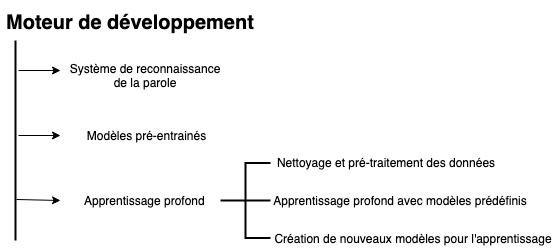
\includegraphics[width=400pt]{images/chap3/Pipeline_moteur_V1.png}
     \caption{Principales fonctions de l'environnement de développement pour la reconnaissance de la parole}
     \label{pip_dev}
 \end{figure}

Nous détaillons dans le chapitre suivant les différents modules de l'environnement de développement ainsi que leur fonctionnement.


\section{Collecte et pré-traitement des données}
Afin d'entraîner un modèle pour la tâche de reconnaissance de la parole, de grandes ressources en terme de données sont requises. Nous nous sommes inspirés des travaux de \cite{e2earabiclexiconfree} afin d'accéder à des données utilisables pour l'apprentissage de notre modèle.\\
Avant de parler de l'extraction et du pré-traitement de ces données, il est important de définir les critères \cite{towardse2esr} que doivent remplir ces dernières pour l'apprentissage. Nos données doivent obligatoirement : 
\begin{itemize}
    \item contenir des enregistrements audio et les transcriptions qui y correspondent,
    \item être de l'arabe moderne standard et non pas un dialecte,
    \item contenir un minimum d'une vingtaine d'orateurs, et
    \item être d'une longueur d'au moins 500 heures de dialogue. \\
\end{itemize}

Pour la conception de notre solution, nous testons nos modèles sur différentes tailles de corpus comme nous l'expliquons dans la suite de ce chapitre. Ces corpus sont respectivement constitués de : six heures de dialogues, 60 heures de dialogue, 260 heures de dialogue et 1200 heures de dialogue. Nous nommons corpus d'essai les six heures de dialogue car la source de données pour ce corpus est différente de celle du reste des données; nous nommons ce second corpus corpus élargi. 

\subsection{Collecte du corpus d'essai}\label{corpus_essais}
Les six heures de dialogue du corpus d'essai furent une partie du corpus collecté par l'équipe QCRI\footnote{https://www.qcri.org} et est disponible en libre accès sur la plateforme Github \cite{qcri6}. De cette référence, nous tirons un fichier texte contenant une liste de liens où chacun correspond à un enregistrement audio. Il a donc fallu développer un algorithme d'extraction automatique pour télécharger ces enregistrements. Nous avons également accès à un fichier contenant la transcription associée à chaque enregistrement. \\
La figure \ref{QCRI6} résume ce processus d'extraction :

\begin{figure}[H]
    \centering
    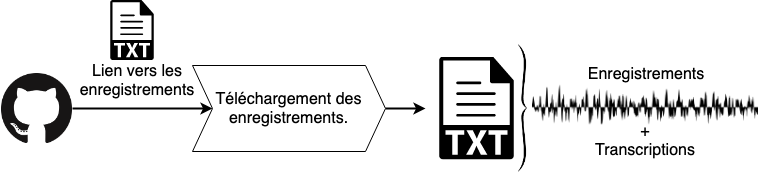
\includegraphics[height=140pt,width=450pt]{images/chap3/QCRI-6h-Github.png}
    \caption{Processus d'extraction des six heures de dialogue du corpus d'essai}
    \label{QCRI6}
\end{figure}

Le résultat est un corpus composé de 2219 enregistrements d'Arabe Moderne Standard (Modern Standard Arabic, MSA) enregistrés par une dizaine d'orateurs et où chaque enregistrement est d'une durée qui varie entre six secondes et une minute environ.

\subsection{Collecte des données du corpus élargi}\label{collecte_donnees}
Pour la suite de la conception du système, nous avons contacté l'équipe du QCRI qui nous ont accordé un accès au corpus MGB-2 \cite{mgb2corpus}. Ce corpus se compose de 1200 heures et plus d'une centaine d'orateurs de programmes enregistrés de la chaîne télévisée Al-Jazeera. La distribution des orateurs est diverse en terme de genre. La plupart de ces programmes sont des interviews de différentes personnalités et contiennent donc des questions. Il est très important pour nous que le corpus contienne des questions. En effet, \textit{ASeR-System} doit retranscrire ce type d'entrées pour qu'il soit testé, par la suite, avec un système de questions-réponses.  Tous les programmes ont été sous-titrés manuellement. 

Contrairement aux données du corpus d'essai, celles du corpus élargi sont formalisées d'une manière différente. La première chose que nous remarquons est les tailles des enregistrements qui sont d'une durée qui varie entre 25 et un peu plus d'une heure. La seconde est le format des fichiers qui contiennent les transcriptions qui sont au format XML suivant l'arborescence suivante : \\

\begin{figure}[H]
    \centering
    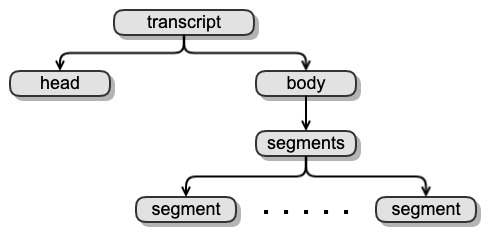
\includegraphics[height=150pt,width=325pt]{images/chap3/xml.jpg}
    \caption{Structure des fichiers XML du corpus élargi contenant les transcriptions}
    % Ancien Titre : Format des fichiers XML contenant les transcriptions
\end{figure}

Afin de tirer partie de ces données, un pré-traitement est nécessaire. Nous découpons ce pré-traitement en : 
\begin{itemize}
    \item extraction des temps de début et de fin de chaque phrase prononcée par un orateur à partir du fichier XML,
    \item extraction de la transcription associée à chaque phrase prononcée par un orateur,
    \item découpage des enregistrements audio selon les temps de début et de fin de phrase, et
    \item constitution d'un corpus contenant des enregistrements de durée allant de 6 à 40 secondes environ ainsi que la transcription qui y est associée sous forme de fichiers texte. \\
\end{itemize}

L'algorithme \ref{algo1} résume l'opération de collecte de données à partir du corpus élargi : 


\begin{algorithm2e}[H]
\SetAlgoLined
\label{ext_trans}
\SetKwInOut{Input}{Input}
\SetKwInOut{Output}{Output}
\Input{     repertoire\_dataset}
\tcc{repertoir\_dataset : le chemin vers le répértoire du dataset}
\Output{\tcc{Pas de variables en Output}}
\BlankLine
 liste\_pairs\_audio\_transcriptions $\gets$ liste\_fichiers(repertoire\_dataset) \\
 \For{(audio, fichierXML) $\in$ liste\_pairs\_audio\_transcriptions}{
    \For{segment $\in$ fichierXML}{
        date\_debut $\gets$ attribut\_start\_time \\
        date\_fin $\gets$ attribut\_end\_time \\
        transcription $\gets$ generer\_transcription(segment) \\
        liste\_transcriptions.ajouter(trancription)
        }
    generer\_fichier\_transcriptions(liste\_transcriptions) \\
    liste\_enregistrements\_audio $\gets$ Decouper\_audio(audio, date\_debut, date\_fin)\\
    generer\_fichier\_audio( liste\_enregistrements\_audio) 
    }
\caption{Extraction des transcriptions et partitionnement des longs enregistrements \label{algo1}}
\end{algorithm2e}

Maintenant que nous avons ces données à notre disposition, nous pouvons passer au pré-traitement pour qu'elles puissent être utilisées lors de l'apprentissage de nos modèles.

\subsection{Pré-traitement des données}
\subsubsection{Extraction des caractéristiques des enregistrements}\label{mfcc_section}
Afin d'utiliser nos enregistrements audio pour la phase d'apprentissage, nous devons extraire les caractéristiques de ces derniers. Il existe différentes manières d'effectuer cette opération mais dans le cadre de la reconnaissance de la parole nous nous intéressons aux caractéristiques MFCC. MFCC est l'acronyme de Mel Frequency Ceptral Coefficient introduit dans les années 1980s \cite{mfccintro}. Le processus par lequel il faut passer pour obtenir les caractéristiques MFCC est le suivant :
\begin{enumerate}[label=(\roman*)]
    \item Le signal audio passe par un filtre de pré-accentuation pour être découpé en un ensemble de spectres (qui peuvent être considérés comme des images ou plutôt des trames).
    \item Une transformation de fourrier est ensuite appliquée à chaque image afin de calculer les fréquences des spectres qui sont appelés périodogrammes.
    \item Calcul des Filter Bank\footnote{Filter Bank : Ensemble de 40 filtres appliqués aux periodogrammes pour extraire les bandes de fréquences.} est effectué pour y appliquer ensuite une Transformée en Cosinus Discrète (TCD) aux groupes de filtres en conservant un certain nombre de coefficients résultants tandis que les autres sont ignorés.
    \item L'étape finale consiste à normaliser les valeurs de ces coefficients.\\
\end{enumerate}

Dans notre cas, après application du MFCC sur nos données, chaque enregistrement audio sera représenté par une matrice de 40 colonnes où chaque colonne est une caractéristique et chaque ligne est une partie du spectrogramme; nous appelons cette partie timestep. Cette matrice n'étant pas normalisée, nous passons par une étape de normalisation.

\subsubsection{Normalisation des spectrogrammes}\label{normalisation_section}
La normalisation des données est une phase quasi nécessaire pour toute tâche d'apprentissage automatique et notre problématique ne fait pas exception à la règle.\\
Il existe plusieurs méthodes pour normaliser un jeu de données; nous nous intéressons à la méthode \textit{Min-Max} qui consiste à calculer les valeurs minimum et maximum de chaque attribut du jeu de données pour ensuite appliquer la formule : 

    \begin{equation}
            Normalise(X_{i}) = \frac{X_{i} - Min(X)}{Max(X) - Min(X)}
            \label{normalisation_equation}
    \end{equation}
    où :\\ \\
    X : est un attribut du spectrogramme, et \\
    $X_{i}$ : une valeur de X que nous voulons normaliser.

Dans le cas de notre problématique, le but de cette normalisation est de contenir toutes les valeurs entre 0 et 1 pour assurer une meilleure mise à jour des poids des réseaux de neurones lors de l'apprentissage.

\subsubsection{Pré-traitement des transcriptions}\label{trans_preprocessing}

Le second volet de nos données est l'ensemble des transcriptions. Chaque transcription est un texte écrit en utilisant la translittération Buckwalter \cite{buckwalter}. Cette translittération définit un mapping non ambigu de représentation de texte arabe en caractères latins étendus et vice-versa. La première étape du pré-traitement consiste à remplacer les caractères présents dans les transcriptions et qui ne font pas partie de l'alphabet Buckwalter. Ces caractères sont les suivants : 
\begin{itemize}
    \item les nombres présents sous la forme de nombres arabes (écrits en graphie occidentale ou orientale) qu'il faut convertir en texte,
    \item le cas particulier des lettres de l'alphabet où certaines lettres qui devraient être en minuscule selon la table Buckwalter sont écrites en majuscule et où une conversion est nécessaire,
    \item le caractère "\%" qui doit être remplacé par des caractères alphabétiques, ainsi que
    \item les caractères "\#", ";", "@" et "\textbackslash \textbackslash" qui n'apparaissent qu'un nombre dérisoire de fois sur tout le jeu de données.\\
\end{itemize}

Ce traitement des caractères spéciaux est important car des caractères superflus et sémantiquement redondants mais syntaxiquement différents augmentent la dimensionnalité des transcriptions. Ceci peut résulter par la suite en un sous-apprentissage. Notons ici, qu'a fin de pouvoir utiliser ces transcriptions lors de l'apprentissage, une conversion vers des valeurs numériques est requise. De ce fait nous présentons deux types d'encodage : encodage basé caractères et encodage basé mots.

\subsubsection{Encodage des transcriptions basé caractères} \label{character_based}
La première étape de cet encodage consiste à attacher au début de la transcription le caractère spécial "\textbackslash t" et le caractère spécial "\textbackslash n" pour marquer le début et la fin de transcription, respectivement.

La conversion de chaque caractère en valeur numérique se fait en utilisant une table de mappage qui associe à chaque caractère une valeur selon l'ordre d'apparition de celui-ci dans le corpus de transcriptions. Maintenant que chaque transcription est sous forme de valeurs numériques, nous appliquons un encodage appelé \textit{One Hot Encoding} \cite{textencoding} qui consiste à représenter chaque transcription sous forme de matrice binaire où chaque ligne représente un caractère de la transcription et où chaque colonne représente un caractère du jeu de caractères du corpus. Il s'agira par la suite de mettre à 1 chaque croisement de caractères entre lignes et colonnes. Pour illustrer cet encodage nous prenons l'exemple suivant : 

Soit le jeu de caractères "a", "b", "x", "d", "e", "l", "o", "h", "r", "w", " " et la phrase "hello world" que nous voulons encoder. La figure \ref{One-hot-car} montre l'encodage One Hot de cette phrase.

\begin{figure}[H]
    \centering
    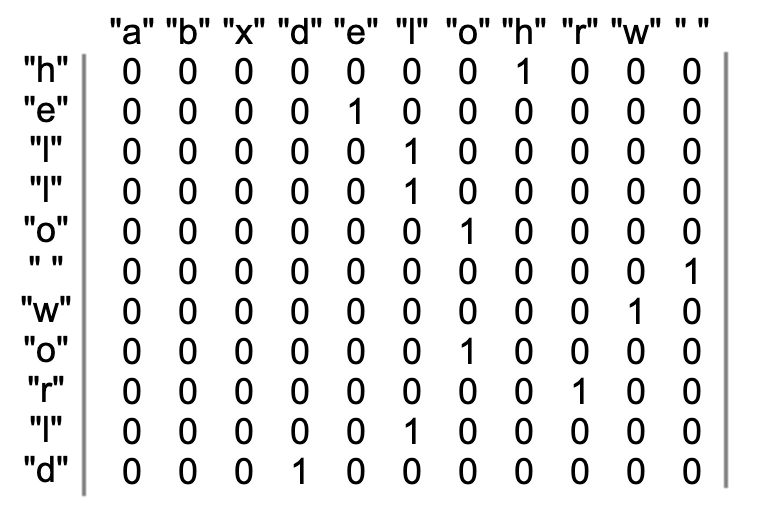
\includegraphics[height=200pt,width=300pt]{images/chap3/matrice_one_hot.png}
    \caption{Exemple de l'encodage basé caractères appelé One Hot Encoding}
    \label{One-hot-car}
\end{figure}

L'algorithme \ref{algo2} résume l'encodage basé caractères des transcriptions :

\begin{algorithm2e}[H]
\SetAlgoLined
\SetKwInOut{Input}{Input}
\SetKwInOut{Output}{Output}
\Input{repertoire\_dataset \\ char\_to\_int\_characters : table de conversion des caractères vers des entiers}
\Output{\tcc{Pas de variables en Output}}
\BlankLine
 liste\_transcriptions $\gets$ recuperer\_transcriptions(repertoire\_dataset) \\
 \For{transcritpion $\in$ liste\_transcriptions}{
    \For{index, caractere $\in$ transcription}
    {
        encoder\_caractere\_en\_input() \\
        \If{index > 1}{
            encoder\_caractere\_en\_target()} \\
    }
    decoder\_input.ajouter(caractere\_encode\_en\_input) \\
    decoder\_target.ajouter(caractere\_encode\_en\_target)
    }
 enregistrer\_fichier(decoder\_input) \\
 enregistrer\_fichier(decoder\_target)
 \caption{Encodage basé caractères des transcriptions \label{algo2}}
 \label{enc_car}
\end{algorithm2e}

L'encodage basé caractères est simple à implémenter mais présente des résultats qui sont moins performants qu'un encodage basés mots. En effet, des erreurs dans les suites de caractères donneraient naissance à des mots qui n'existent pas. C'est pour cela qu'il faut y associer un modèle de langage pour corriger ces erreurs. L'encodage basé mots quant à lui, en plus de présenter des résultats plus cohérents que ceux de l'encodage basé caractères, fait office de modèle de langage en assurant que les suites de caractères sont correctes pour les mots prédits correctement.

Nous présentons dans ce qui suit les différentes approches pour l'encodage basé mots.
 

\subsubsection{Encodage des transcriptions basé mots}\label{word_based}
Tout comme pour l'encodage basé caractères, nous attachons au début de nos transcriptions le mot spécial SOS qui signifie "Start Of Sentence" et à la fin le mot EOS qui signifie "End Of Sentence" pour marquer respectivement le début et la fin d'une transcription.

L'encodage basé mots va vraisemblablement présenter des résultats très différents de l'encodage basé caractères et ce car le modèle devra distinguer et classifier un très grand nombre de mots en comparaison avec une cinquantaine de caractères pour le premier encodage. 

Pour encoder des mots,  nous pensons naturellement à l'encodage \textit{One Hot Encoding} également appelé \textit{Bag Of Words} dans le cas des mots. C'est une approche similaire à celle présentée dans la section  \ref{character_based} et qui consiste à représenter une transcription par une matrice où les lignes représentent les mots, séparés par le caractère blanc, et les colonnes représentent tous les mots distincts de notre jeu de données. Nous illustrons cet encodage par un exemple réel de notre jeu de données. Prenons la phrase "m\$AhdynA AlkrAm AlslAm Elykm" qui est la translittération de "\setcode{utf8}\<مشاهدينا الكرام السلام عليكم>" dont l'encodage est le suivant :  

\begin{figure}[H]
    \centering
    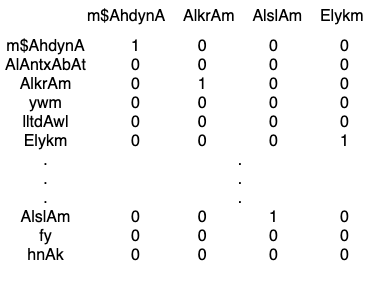
\includegraphics[height=200pt,width=300pt]{images/chap3/One-Hot-Word-level.png}
    \caption{Exemple de l'encodage basé mots Bag Of Words}
    \label{exemple_bag_of_words}
\end{figure}

Cet encodage paraît adéquat à première vue mais pour un jeu de données aussi large que le notre où il existe plus de 150000 mots distincts, il est quasi-impossible, en terme de mémoire vive, d'encoder chaque transcription \textit{x} sous forme d'une matrice de taille (x, 150000) d'où l'impossibilité d'utiliser cet encodage pour notre dataset.

Il existe néanmoins un autre encodage qui est l'encodage binaire où nous convertissons chaque mot en vecteur binaire. Cet encodage s'effectue en suivant les étapes suivantes :
\begin{itemize}
    \item Collecte de la liste des mots distincts existant dans notre jeu de données.
    \item Création d'une table associant un indice unique à chaque mot.
    \item Création d'un vecteur binaire avec une taille suffisante pour encoder chaque indice tel que :
    \begin{equation}
        2^{x} < nbr\_mots\_distincts
    \end{equation}
    où :\\ \\
    $x$ est le nombre de bits du vecteur.
    Nous estimons ne pas avoir besoin de plus de 18 bits pour encoder chaque mot de notre jeu de données.
    \item Convertir l'indice de chaque mot en binaire et l'introduire dans le vecteur binaire. \\
\end{itemize}

Si nous prenons l'exemple précédent avec la phrase : "m\$AhdynA AlkrAm AlslAm Elykm", l'encodage de cette dernière serait le suivant : 

\begin{figure}[H]
    \centering
    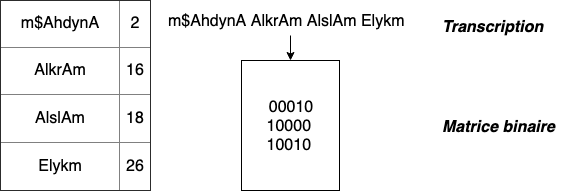
\includegraphics[width=400pt]{images/chap3/Binaire.png}
    \caption{Encodage binaire des mots du jeu de données}
\end{figure}

Bien que l'encodage binaire semble apporter la solution à notre problématique, il présente un désavantage majeur lors de l'apprentissage qui est le calcul d'une fausse précision. Si pour un vecteur binaire le modèle nous affiche, par exemple, une précision de 90\%, notre modèle aura donc la faculté de prédire 9 bits sur 10 mais après reconversion du vecteur binaire prédit en mot nous nous rendrons compte que le mot deviendra un tout autre mot.

Afin de remédier à cette anomalie, nous présentons un nouvel encodage pour les mots. Le principe de cet encodage consiste à :
\begin{itemize}
    \item calculer le nombre maximum de caractères par mot dans notre jeu de données,
    \item pour les transcriptions en entrée du modèle d'apprentissage, encoder chaque mot d'une transcription par un vecteur de taille \textbf{\og Nombre de caractères du jeu de données $\times$ Nombre maximum de caractères par mot \fg} de telle sorte à encoder chaque caractère de chaque mot en utilisant un One Hot Encoding sur une partie de taille \textbf{{Nombre de caractères du jeu de données}} de ce vecteur, et
    \item pour les transcriptions en sortie du modèle d'apprentissage, encoder chaque mot de la transcription par \textbf{N} vecteurs où \textbf{N} représente le \textbf{nombre maximum de caractères par mot} et où chaque vecteur est de taille \textbf{\og Nombre de caractères du jeu de données \fg}.\\ 
\end{itemize}

Afin de clarifier cet encodage qui peut paraître inhabituel au premier abord, nous présentons un exemple d'encodage avec le mot "hello", le jeu de caractères "a", "e", "h", "l", "b", "x", "o", " " et la taille maximale de mots de 7 comme le montre la figure \ref{word_based_multiple_output}.

 \begin{figure}[H]
    \centering
    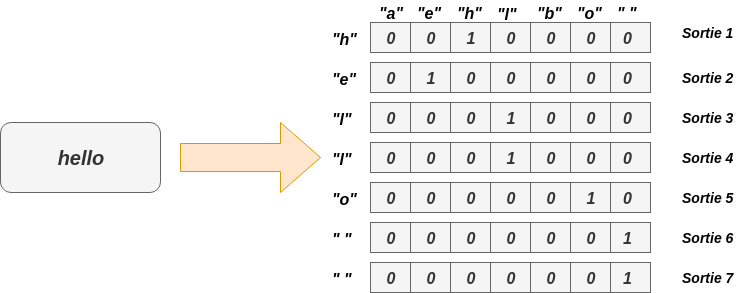
\includegraphics[height=175pt,width=350pt]{images/chap3/encodage_base_mots.png}
    \caption{Exemple Encodage basé mots à plusieurs sorties}
    \label{word_based_multiple_output}
\end{figure}

L'algorithme \ref{algo3} suivant résume cet encodage :

\begin{algorithm2e}[H]
\SetAlgoLined
\SetKwInOut{Input}{Input} 
\SetKwInOut{Output}{Output} 
\Input{repertoire\_dataset \\ char\_to\_int\_characters : table de conversion des caractères vers des entiers \\ max\_car\_mot : maximum de caracteres par mot de tout le corpus \\ nb\_car : nombre de caracteres disctincts du corpus}
\Output{\tcc{Pas de variables en Output}}
\BlankLine
liste\_transcriptions $\gets$ recuperer\_transcriptions(repertoire\_dataset) \\
\For{transcritpion $\in$ liste\_transcriptions}{
    liste\_mots $\gets$ diviser\_transcription\_en\_mots(transcription) \\
    \For{ mot $\in$ liste\_mots}{
        longueur\_liste $\gets$ nb\_car $\times$ max\_car\_mot \\
        encoded\_word $\gets$ liste\_de\_zeros(longueur\_liste) \\
        encoded\_word\_target $\gets$ matrice\_de\_zeros(nbr\_car, max\_car\_mot) \\
        \For{i, index\_caractere $\in$ mot}{
            encoder\_caractere\_en\_input()\\
            \If{i<max\_caracteres\_par\_mot}{
                encoder\_fin\_mot\_input()
                \If{i > 1}{
                encoder\_caractere\_en\_target() \\
                } 
            }
        }
        
    }
    encoded\_input.ajuoter(encoded\_transcriptions\_input) \\
    encoded\_target.ajouter(encoded\_transcriptions\_target) 
}
enregistrer\_fichier(decoder\_input) \\
enregistrer\_fichier(decoder\_target) 
\caption{Encodage basé mots des transcriptions \label{algo3}}
\label{enc_mot}
\end{algorithm2e}

En adoptant un tel encodage, nous évitons les difficultés liées à la gestion de la mémoire ainsi que l'erreur entre la précision et le WER pour l'encodage binaire. Nous présentons dans le chapitre suivant l'implémentation d'un tel encodage ainsi que les performances achevées par ces deux encodages. 

\subsubsection{Teacher Forcing}
Afin de mettre en place l'architecture que nous présentons dans la suite de ce chapitre, nous aurons, en plus des transcriptions encodées, une copie encodée de ces transcriptions à l'instant t+1. Ce principe s'appelle Teacher Forcing \cite{teacherforcing}, également appelé Professor Forcing. Cela permet à notre système de déduire quel caractère/mot avoir en sortie sachant  l'enregistrement audio et la séquence de caractères/mots précédents.

\subsubsection{Traitement des grandes tailles de données}
Comme mentionné précédemment, nous aurons à effectuer notre apprentissage sur des jeux de données de tailles différentes afin d'évaluer les performances des différents modèles. Nous serons donc amenés à effectuer des apprentissages sur six heures, 60 heures, 260 heures et 1200 heures d'enregistrements audio en fin de parcours.

Gérer une telle quantité de données nous met face à deux problèmes principaux : 
\begin{itemize}
    \item impossibilité de charger le dataset nettoyé en mémoire pour l'encodage des transcriptions au vue de sa taille, et
    \item envoi de toutes les données à notre modèle pour l'apprentissage sachant que dix heures de dialogue équivaut à environ 500 Mo en mémoire. \\
\end{itemize}

Afin de remédier à ces complications, nous appliquons le principe de pagination. Nous commençons par la génération des fichiers binaires qui contiennent les spectrogrammes ainsi que leurs transcriptions. Au lieu de générer un fichier contenant toutes les données à notre disposition, nous générons un ensemble de fichiers en limitant le nombre d'heures de dialogue contenues dans chaque fichier. Nous prenons, pour la suite de ce projet, des fichiers de dix heures de dialogue chacun.

L'étape suivante consiste à créer à partir de ces partitions, des sous-partitions de telle sorte à avoir des fichiers binaires pour l'apprentissage et le test. Nous définissons ce nombre de sous-partitions de manière dynamique de telle sorte à avoir une utilisation minimum de la mémoire vive de l'utilisateur. Nous calculons le nombre de partitions à partir de la formule suivante : 
\begin{equation}
    nbr\_partitions = \frac{32}{memoire\_utilisateur} * duree\_dataset\_heures
\end{equation}

Nous rencontrons une difficulté supplémentaire lors de l'apprentissage car nous devons envoyer toutes nos données à notre modèle pour qu'il puisse effectuer la mise à jour des poids sur l'ensemble de données mais là nous ne pouvons avoir toutes nos données en mémoire. C'est ici que nous faisons appel au principe de générateur de données qui se définit par les étapes suivantes : 

\begin{itemize}
    \item création d'une fonction chargeant en mémoire, à tour de rôle, les couples de fichiers contenant les spectrogrammes et transcriptions,
    \item création d'une table de hachage contenant comme clé les couples de nombre de timesteps des spectrogrammes et transcriptions, et comme valeur une liste des spectrogrammes et transcriptions ayant ces tailles, et
    \item envoi successif des listes de chaque clé à la fonction d'apprentissage.
\end{itemize}

Nous avons donc implémenté manuellement l'envoi des données à la fonction d'apprentissage pour permettre une gestion optimale de la mémoire en premier lieu et d'accélérer l'apprentissage en second lieu.

Maintenant que notre corpus est extrait et pré-traité nous passons à la conception des différentes architectures de modèles pour notre système.


\section{Apprentissage du système}\label{apprentissage}
Nous nous attelons dans cette partie à la conception du modèle de notre système de reconnaissance de la parole. Comme mentionné précédemment, nous développons un système End-To-End qui, contrairement à l'approche basée reconnaissance de phonèmes, consistera en un module prenant en entrée un enregistrement audio et fournissant en sortie la transcription qui lui correspond. Dans le cas de la reconnaissance de la parole, nous avons affaire à des données de type séries temporelles où la taille de chaque enregistrement est variable. Comme tout exercice d'apprentissage, il existe plusieurs modèles et plusieurs architectures pour appréhender le problème. Pour les séries temporelles, nous nous intéressons aux modèle de type Séquence à Séquence.

\subsection{Séquence à Séquence et Encodeur/Décodeur}
Le modèle Séquence à Séquence, traduit de l'anglais Sequence to Sequence, fut introduit en 2014 par Google \cite{seq2seqgoogle}. Ce modèle a pour but de mapper une entrée avec une sortie et où la longueur des entrées et celle des sorties peuvent être différentes.

Par exemple, traduire "What are you doing today ?" de l'anglais vers le français comporte une entrée de 5 mots et une sortie de 4 mots "Que faites-vous aujourd'hui ?". Comme les tailles des entrées et sorties sont différentes, ce qui est le cas pour les problèmes à données sous forme de séquences, nous ne pouvons utiliser un architecture séquentielle classique pour mapper chaque mot de la phrase en anglais à la phrase en français. Le modèle séquence à séquence est utilisé pour traiter des problèmes comme celui-ci.

Le modèle séquence à séquence se base sur le principe sous-jacent d'encodeur/décodeur \cite{encdecdef} que nous représentons par l'illustration suivante :
\begin{figure}[H]
    \centering
    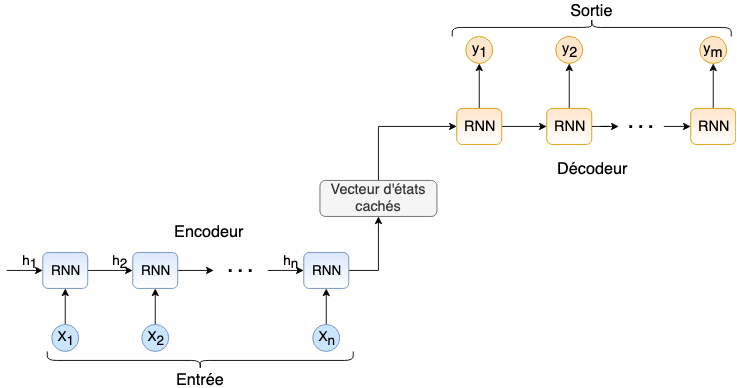
\includegraphics[height=200pt,width=400pt]{images/chap3/EncDec.png}
    \caption{Architecture de base d'un encodeur/décodeur}
    \label{Enc_Dec}
\end{figure}

Comme illustré dans la figure \ref{Enc_Dec}, le modèle comprend deux blocs principaux qui sont l'encodeur et le décodeur ainsi qu'un vecteur intermédiaire qui est le vecteur d'états cachés.


\subsubsection{Encodeur}
L'encodeur est le premier bloc de ce modèle et est composé d'une pile de plusieurs unités récurrentes. Chacune de ces unités ne prend qu'un timestep de la séquence d'entrée et collecte les informations relatives à cet élément que nous appelons état caché (hidden state en anglais) et qui se calcule à partir de la formule suivante :

\begin{equation}
    h_{t} = f(W^{(hh)}h_{t-1} + W^{(hx)}x_{t})
\end{equation}
    où :\\ 
    h : est l'état caché à timestep \textit{t}. \\
    x : est la donnée à un pas de temps \textit{t}. \\
    $W^{(hh)}$ : représente les poids relatifs l'état caché.\\
    $W^{(hx)}$ : représente les poids relatifs à la sortie de l'encodeur.

L'encodeur a pour but de donner une représentation de la séquence de données afin de "l'encapsuler" dans le vecteur d'états cachés (Hidden States Vector en anglais), et va donc contenir l'état caché final produit par l'encodeur du modèle qui fera office d'état initial pour le décodeur.

Dans le cadre de notre projet, l'encodeur est la partie du modèle qui prend les enregistrements audio en entrée et apprend à regrouper les séquences d'un spectrogramme et produire une représentation vectorielle de celle-ci.

\subsubsection{Décodeur}
Tout comme l'encodeur, le décodeur se compose d'un ensemble d'unités récurrentes \cite{encoderdecoder} où : 
\begin{itemize}
    \item chaque unité prédit une sortie \textbf{$Y_{t}$} pour un pas de temps \textbf{t}, et
    \item chaque unité prend en entrée la donnée et un vecteur d'état caché de l'unité précédente (ou de l'encodeur si c'est la première unité) et génère à partir de cela un output et son propre vecteur d'états cachés pour l'unité suivante.\\
\end{itemize}

Le calcul de l'état caché se fait à partir de la formule suivante :

\begin{equation}
    h_{t} = f(W^{hh}h_{t-1})
\end{equation}
    où :\\ 
    h : est l'état caché à un pas de temps t. \\
    $W^{(hh)}$ : représente les poids du réseau.
    
et l'output {$Y_{t}$} de l'unité récurrente pour un pas de temps \textbf{t} est calculé à partir de l'état caché selon la formule suivante :
\begin{equation}
    Y_{t} = Softmax(W^{s}h_{t})
\end{equation}
où :\\
    Y : est l'output de l'encodeur à un pas de temps t. \\
    h : est l'état caché à un pas de temps t. \\
    W : représente les poids du réseau. \\
    \textit{Softmax} : est une fonction d'activation qui attribue des probabilités décimales à chaque classe d'un problème à plusieurs classes. La somme de ces probabilités décimales doit être égale à 1 \cite{softmax}.

\subsection{Discussion}
L'intérêt du modèle encodeur/décodeur réside dans le fait de pouvoir associer des séquences de différentes longueurs en entrée et en sortie. Nous utilisons ce modèle pour le développement du système où :
\begin{itemize}
    \item les entrées de l'encodeur sont nos enregistrements audio,
    \item les entrées du décodeur sont les transcriptions, et
    \item les sorties du décodeur sont les transcriptions à \textit{t+1} selon le principe de Teacher Forcing que nous détaillons dans le chapitre suivant. \\
\end{itemize}

Nous passons à présent à la conception de l'architecture interne des unités récurrentes de notre modèle.

\section{Architecture du modèle}
Il existe plusieurs architectures possibles pour le développement de notre modèle, comme nous l'avons noté dans l'état de l'art. Chaque travail trouvé dans l'état de l'art présente une conception, un corpus et bien évidement des résultats différents, ce qui peut prêter à confusion.

Afin de mettre en place l'architecture idéale pour notre modèle, nous en expérimentons deux et pour chaque architecture nous prenons en compte deux variantes. Nous comparons ensuite l'évolution des courbes d'apprentissage de chaque architecture. Afin que notre système soit améliorable, il doit pouvoir prendre en compte l'augmentation (ou même la réduction) du volume de données. Ainsi, pour que cette comparaison soit précise, nous utilisons quatre jeux de données : six heures de dialogue, 60 heures, 260 heures et 1200 heures de dialogue.

Avant de présenter nos architectures nous commençons par présenter les couches que nous utilisons.

\subsection{Présentation des couches utilisées}
\subsubsection{Long Short-Term Memory}
Long-Short-Term-Memory, ou LSTM, sont un type particulier de RNNs et ont été introduits par \cite{lstmdef}. Les LSTMs ont été conçus pour éviter le problème de dépendance à long terme. En effet, il s'est avéré que les RNNs ne peuvent apprendre le séquencement d'informations à long terme. Comprendre et se souvenir du séquencement des informations quelque soit la taille de la séquence est l'avantage des LSTMs par rapport aux RNNs, et ce grâce au mécanisme des portes présentes dans une cellule LSTM. Ces portes peuvent apprendre les données importantes à conserver parmi les données d'entrée. En faisant cela, un LSTM peut transmettre des informations pertinentes tout au long de la séquence de données pour effectuer des prédictions.

La figure \ref{LSTM} présente le contenu d'une cellule LSTM ainsi que les opérations internes qu'y s'effectuent : 

\begin{figure}[H]
    \centering
    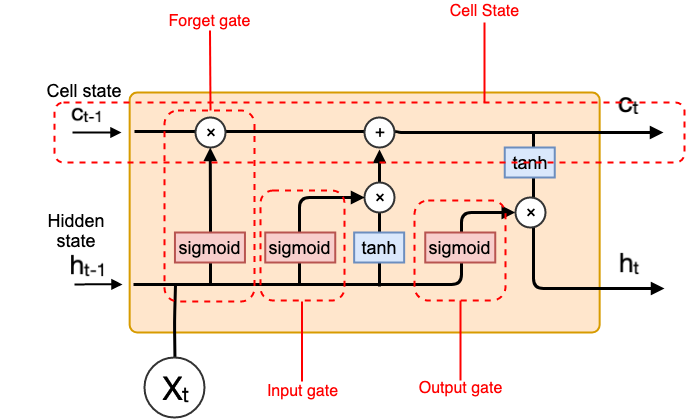
\includegraphics[height=190pt,width=325pt]{images/chap3/LSTM.png}
    \caption{Contenu d'une cellule LSTM \cite{LSTM_cell}}
    \label{LSTM}
\end{figure}

Comme le montre la figure \ref{LSTM}, en plus du Hidden State qu'on retrouve dans une cellule RNN, il y a le Cell State qui est le concept de base des LSTMs. Le Cell State permet de garder en mémoire les informations pertinentes. Ces informations sont donc sauvegardés grâce aux trois portes d'une cellule LSTM \cite{lstmgates} qui sont :

\begin{itemize}
    \item \textbf{Forget Gate} : pouvant être traduite en porte d'oubli, elle décide quelles informations doivent être conservées. Pour se faire, les informations contenus dans le vecteur d'états cachés précédent et les données en entrée sont additionnées et passent par la fonction sigmoïde et la valeur résultante est comprise entre 0 et 1. Plus la valeur se rapproche de 1 plus l'information est pertinente.\\
    \item \textbf{Input Gate} : L'input Gate, ou porte d'entrée, permet de mettre à jour le Cell State. Les valeurs du vecteur d'états cachés précédent et celles des donnée en entrée sont additionnées et passent par une fonction sigmoïde ce qui, comme pour la Forget Gate, permet de désigner les données pertinentes. En plus de la fonction sigmoïde, ces mêmes informations passent par une fonction tanh pour rendre les valeurs entre -1 et 1 afin de contribuer à la régulation du réseau. Les sorties de la fonction sigmoïde ainsi que tanh sont multipliées et ce résultat est additionné à la valeur contenue dans le Cell State.\\
    \item \textbf{Output Gate} : l'Output Gate, ou porte de sortie, décide quel devrait être le prochain vecteur d'états cachés. Premièrement, nous passons l'état caché précédent et l'entrée actuelle dans une fonction sigmoïde. Ensuite, nous passons le Cell State mis à jour par la fonction tanh. Nous multiplions la sortie tanh par la sortie sigmoïde pour décider quelles informations l'état caché doit contenir. C'est ainsi que sont générés les nouveaux Cell State et Hidden State qui seront utilisés pour le timestep suivant.
\end{itemize}
        
\subsubsection{Gated Reccurent Unit}
Introduit en 2014 par \cite{GRUpaper}, les Gated Reccurent Units (GRU) sont des unités récurrentes assez similaires à des LSTMs dans leur fonctionnement. Les principales différences sont que les GRUs n'ont pas de Cell State pour transferer l'information et n'ont que deux portes \cite{lstmgates} : 
\begin{itemize}
    \item \textbf{Update Gate} : agit de manière similaire aux Forget Gate et Input Gate d’un LSTM. Cette porte décide quelles informations doivent être gardées et quelles nouvelles informations ajouter; et
    \item \textbf{Reset Gate} : utilisée pour décider de la quantité d'informations à oublier.\\
\end{itemize}

La figure \ref{GRUU} présente le contenu d'une unité GRU ainsi que les opérations internes qu'y s'effectuent.

\begin{figure}[H]
    \centering
    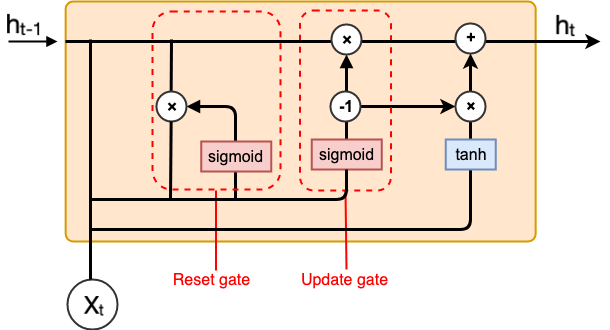
\includegraphics[height=185pt,width=325pt]{images/chap3/GRU.png}
    \caption{Contenu d'une cellule GRU}
    \label{GRUU}
\end{figure}

Les GRUs effectuent moins de calculs matriciels que les LSTMs et sont donc un peu plus rapides lors de l'apprentissage.

\subsubsection{Couches récurrentes bidirectionnelles}
Les couches récurrentes bidirectionnelles sont une extension des RNNs traditionnels qui peuvent améliorer les performances du modèle en cas de problème de classification de séquences \cite{bilstmdef}. Dans les problèmes où tous les timesteps de la séquence d'entrée sont disponibles, comme le cas de notre problème, les RNNs bidirectionnels entraînent deux RNNs au lieu d'un seul. Le premier de ces RNN accomplit un apprentissage sur la séquence d'entrée de la manière usuelle tandis que le second le fait sur une copie triée dans le sens inverse de la séquence d'entrée. Cela peut fournir un contexte supplémentaire au réseau et permettre un apprentissage plus plus complet. Pour notre problématique, ce type de couches joue le rôle d'un modèle de langage. 

\subsection{Architectures de l'approche End-To-End pour ASeR-Sytem}
Nous présentons dans cette partie les deux architectures où chaque architecture est basée sur un modèle encodeur/décodeur avec des RNNs mais aussi une variante à base de RNNs bidirectionnels pour chacune des deux architectures.

\subsubsection{Architecture de base}
Le modèle de base se compose de :
\begin{itemize}
    \item \textbf{Encodeur} : composé d'une couche récurrente et renvoie les vecteur Hidden State.
    \item \textbf{Décodeur} : composé de plusieurs couches récurrentes.
    \item \textbf{Couche Fully Connected} : Dernière couche du modèle d'un réseau de neurones MLP complètement connecté qui prend en entrée l'output du décodeur. \\
\end{itemize}

La figure \ref{Baseline} résume l'architecture de ce modèle.
\begin{figure}[H]
    \centering
    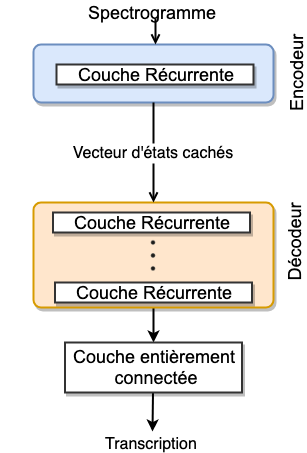
\includegraphics[height=240pt]{images/chap3/baseline_model.png}
    \caption{Architecture de base de ASeR-System}
    \label{Baseline}
\end{figure}

\subsubsection{Architecture avec couches convolutionnelles}
Le modèle à couches convolutionnelles se compose de :
\begin{itemize}
    \item \textbf{Couches convolutionnelles} : Se compose d'un ensemble de convolutionnelles et couches Pooling. Cette partie du modèle a pour but d'extraire les informations pertinentes du spectrogramme et de supprimer le bruit qui aurait échapper aux filtres du MFCC. La dernière couche génère des spectogrammes modifiés qui seront injectés en entrée de l'encodeur.
    \item \textbf{Encodeur} : composé d'une couche récurrente et renvoie le vecteur Hidden State.
    \item \textbf{Décodeur} : composé de plusieurs couches récurrentes. En plus de cela, le décodeur comporte une couche Dropout qui a pour but de minimiser les risques de sur-apprentissage en désactivant aléatoirement certains neurones des couches précédentes.
    \item \textbf{Couche Fully Connected} : Dernière couche du modèle, prend en entrée l'output du décodeur. \\
\end{itemize}

La figure \ref{arch_cnn} résume l'architecture du modèle.
\begin{figure}[H]
    \centering
    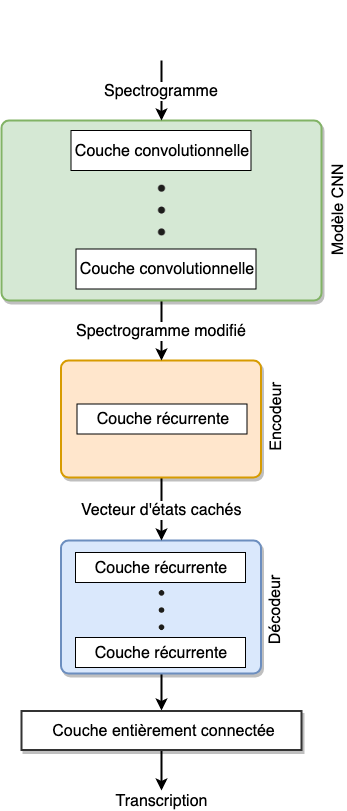
\includegraphics[height=340pt]{images/chap3/CNN_model.png}
    \caption{Architecture de ASeR-System avec couches convolutionnelles}
    \label{arch_cnn}
\end{figure}

\section{Utilisation du modèle d'apprentissage pour la reconnaissance}\label{inference}
Après l'apprentissage de notre modèle, nous devrons tester celui-ci sur des données de test dans un premier temps ensuite des données réelles ou, autrement dit, tester nos propres enregistrements audio. Contrairement à un modèle d'apprentissage classique, le modèle séquence à séquence ne fait pas une simple prédiction de classes qui, dans notre cas, nécessiterait l'enregistrement audio et sa transcription en entrée du modèle. C'est pour cela que nous effectuons une tâche d'inférence
\cite{modelinference}. Nous ne pouvons parler directement de prédiction car notre modèle se compose d'un encodeur et d'un décodeur. Le processus d'inférence se décompose en deux parties : la préparation du modèle après l'apprentissage et le décodage des transcriptions. La préparation du modèle se fait donc comme suit :

\begin{itemize}
    \item Chargement des couches d'entrée et états cachés de l'encodeur à partir du modèle après apprentissage.
    \item Chargement des couches d'entrées, couches récurrentes ainsi que couches de sortie du décodeur.
    \item Génération d'un modèle pour l'encodeur et un modèle pour le décodeur et ce à partir des couches chargés préalablement. \\
\end{itemize}

Maintenant que l'encodeur et le décodeur sont prêts, nous passons au décodage des transcriptions. Il est à noter que cette partie de l'inférence est sensiblement la même pour un encodage basé caractères ou encore un encodage basé mots. Les étapes sont les suivantes : 

\begin{itemize}
    \item Préparation de la table qui associe cette fois un entier à chaque caractère ou mot selon l'encodage.
    \item Prédiction du vecteur d'états cachés à l'aide de l'encodeur. Ce vecteur est la représentation de l'enregistrement audio en entrée.
    \item Prédiction du caractère ou du mot correspondant en donnant en entrée du décodeur le vecteur d'états ainsi que le caractère ou mot actuel, la sortie est le caractère ou mot prédit ainsi qu'un vecteur d'états qui sera en entrée de la prochaine prédiction. Si la prédiction effectuée est celle du premier caractère, le vecteur d'états est le vecteur d'états cachés généré par l'encodeur.
    \item Répéter l'étape précédente tant que le caractère ou mot généré n'est pas fin de transcription.
\end{itemize}

% Nous prenons un exemple réel pour illustrer le principe d'inférence avec la phrase : "yEtbr fyh AlEdyd mn xSwmkm AlsyAsyyn >n hnAk" ainsi qu'un encodage basé caractères. La figure ci-dessous résume les différentes étapes.

% \begin{figure}[H]
%     \centering
%     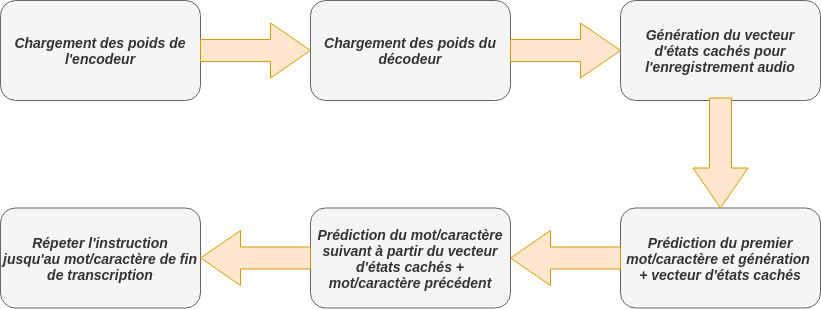
\includegraphics[width=400pt]{images/chap3/inference.png}
%     \caption{Étapes de l'inférence}
% \end{figure}


\section{Application de ASeR-System à un système de questions-réponses} \label{QASChap3}
 \textit{ASeR-System} peut être utilisé dans plusieurs domaines d'application du traitement automatique du langage naturel (TALN). Dans le cadre de ce projet, nous considérons les systèmes de questions-réponses comme domaine d'application. 

 L'équipe du LRIA, laboratoire de recherche en intelligence artificielle (Laboratory for Research in Artificial Inteligence) de l'université des sciences et de la technologie Houari Boumédiène a développé un système de questions-réponses nommé \textit{AFaQ-System} qui a été mis à notre disposition. Comme nous l'avons mentionné dans les sections \ref{QASdomain} et \ref{QASqstType}, un système de questions-réponses peut être classifié selon le domaine et/ou le type de questions qu'il accepte, le système de questions-réponses \textit{AFaQ-System} est de type factoïde, il répond aux questions qui commencent par :   \setcode{utf8}\< متى، كم، أين، من>. Un corpus \cite{QASCorpus} a été exclusivement développé dans le but d'être utilisé pour l'apprentissage des modèles des différents modules de ce système qui se compose de trois modules à savoir : 
 \begin{itemize}
     \item le module de pré-traitement d'une question (Question preprocessing),
     \item le module de pré-traitement des documents (document preprocessing), et
     \item le module d'extraction de réponses (answer extraction). \\
 \end{itemize}

La figure \ref{QAS_ASR} illustre la conception de l'application développée dans le cadre de ce projet. Cette application permet d'utiliser \textit{ASeR-System} avec \textit{AFaQ-System}.
 \begin{figure}[H]
    \centering
    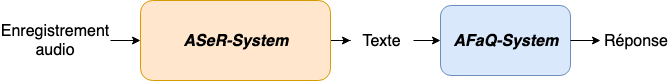
\includegraphics[width=400pt]{images/chap3/QASASR.png}
    \caption{Système de reconnaissance de la parole intégré avec un système de questions-réponses }
    \label{QAS_ASR}
\end{figure}

% dans la presentation on peut parler de l archi du modele sans trop détail : on parle vite fait sur les modules qui composent le QAS : Question processing, document processing et answer extraction 
% type du QAS : factoid (mata kam ayna et man)
% l accuracy par rapport à chaque question (confirmer avec guessoum)
% Le corpus sur le quel le tout à été testé (taille, type de question etc)  voir papier envoyer par aouichat 
% Comment le systeme de QR est integrer --> voir schéma



\section{Conclusion}
Dans de ce chapitre, nous avons présenté les données à notre disposition ainsi que le pré-traitement mis en place afin d'en tirer profit pour l'apprentissage de nos modèles. Ensuite, nous avons présenté au total quatre architectures basées sur le principe d'encodeur/décodeur mais qui se composent de couches différentes. Le but principal de ce choix de conception est de garantir l'implémentation d'un modèle fiable et performant. Pour finir, nous avons présenté \textit{AFaQ-System}, le système de questions-réponses que nous utilisons pour tester \textit{ASeR-System}.

Dans le chapitre suivant, nous passons à l'implémentation de nos modèle ainsi que le pré-traitement des données au vu des différentes phases d'apprentissage. Une fois le choix du modèle effectué sur la base de l'évolution des performance de chaque architecture, nous passerons à l'apprentissage du modèle final et au test de notre système à travers un système de questions-réponses.